\chapter{Methodology}\label{ch:methodology}


\section{Dataset}\label{sec:dataset}
The dataset was the same as in the unpublished study of Hammer et al~\cite{Hammer-2021}.
Modified with the authors permission, the description of the experiment settings, and the pre-processing follows.

\subsection{Movement task and kinematic variables}\label{subsec:movement-task-and-kinematic-variables}
A dataset that was already used in several other iEEG studies to examine decoding of movement kinematic parameters\cite{Hammer-2021,hammer-predominance-2016,hammer-role-2013} was utilized for the purposes of this thesis.
The participants performed a motor task based on driving a car in a computer simulation.
They controlled the position of the car on a computer screen using a steering wheel which they held in both hands.
The task was to keep the car on a curved road.
The road was random without any repetitions, following a low-pass filtered white noise trajectory.
During the movement task, the position of the car on the road was measured.
The position of the car linearly corresponded to the deflection of the steering wheel and was measured relative to the screen center, which corresponded to zero-deflection of the steering wheel.
Importantly, the control of the car's position was possible only in the horizontal dimension (left - right).
The upward movements of the car (vertical scrolling speed) were kept constant in each run of the game and adjusted for each subject individually. \\

The difficulty and the recording time of each subject was also adjusted based on the participant's motivation/ability to participate, lasting $25 \pm 7 min (mean \pm SD$).
The car game difficulty was modified by the vertical scrolling speed of the car.
Therefore, to account for faster movements, the low-pass cutoff frequency was set to 10~Hz for smoothing the raw tracker data prior to the derivation of the kinematic parameters. \\

From the horizontal - 1-D trajectory, the following two kinematic parameters were derived:
1. velocity computed as a derivative of position, 2. speed as the absolute value of velocity.
Velocity thus contained the directional information in its sign;
specifically, velocity values smaller than zero implicated movement to the left and vice versa, while speed indicated how fast the car was moving left or right (irrespective of its direction).
The time-series of the kinematic parameters were resampled at 250~Hz and temporally aligned to the iEEG data.

\subsection{Recording}\label{subsec:recording}
The recordings were performed in the University Medical Centre in Freiburg, Germany and in the Motol University Hospital in Prague, Czech Republic.
The study included 12 epilepsy patients (6 male, age 19--50, $ 33 \pm 10, (mean \pm SD $) all of which had intracranial EEG implantations.
Some of the implantations were placed in the region of the motor cortex.
The location of the electrodes was dependent solely on the needs for medical evaluation of their medication-resistant epilepsy.
Both sEEG and ECoG electrodes were present among patients.
Detailed information about electrode type and placement is presented in Table\ref{tab:patient-table} and Figure\ref{fig:electrodes}.

\begin{figure}[!htbp]
\centering
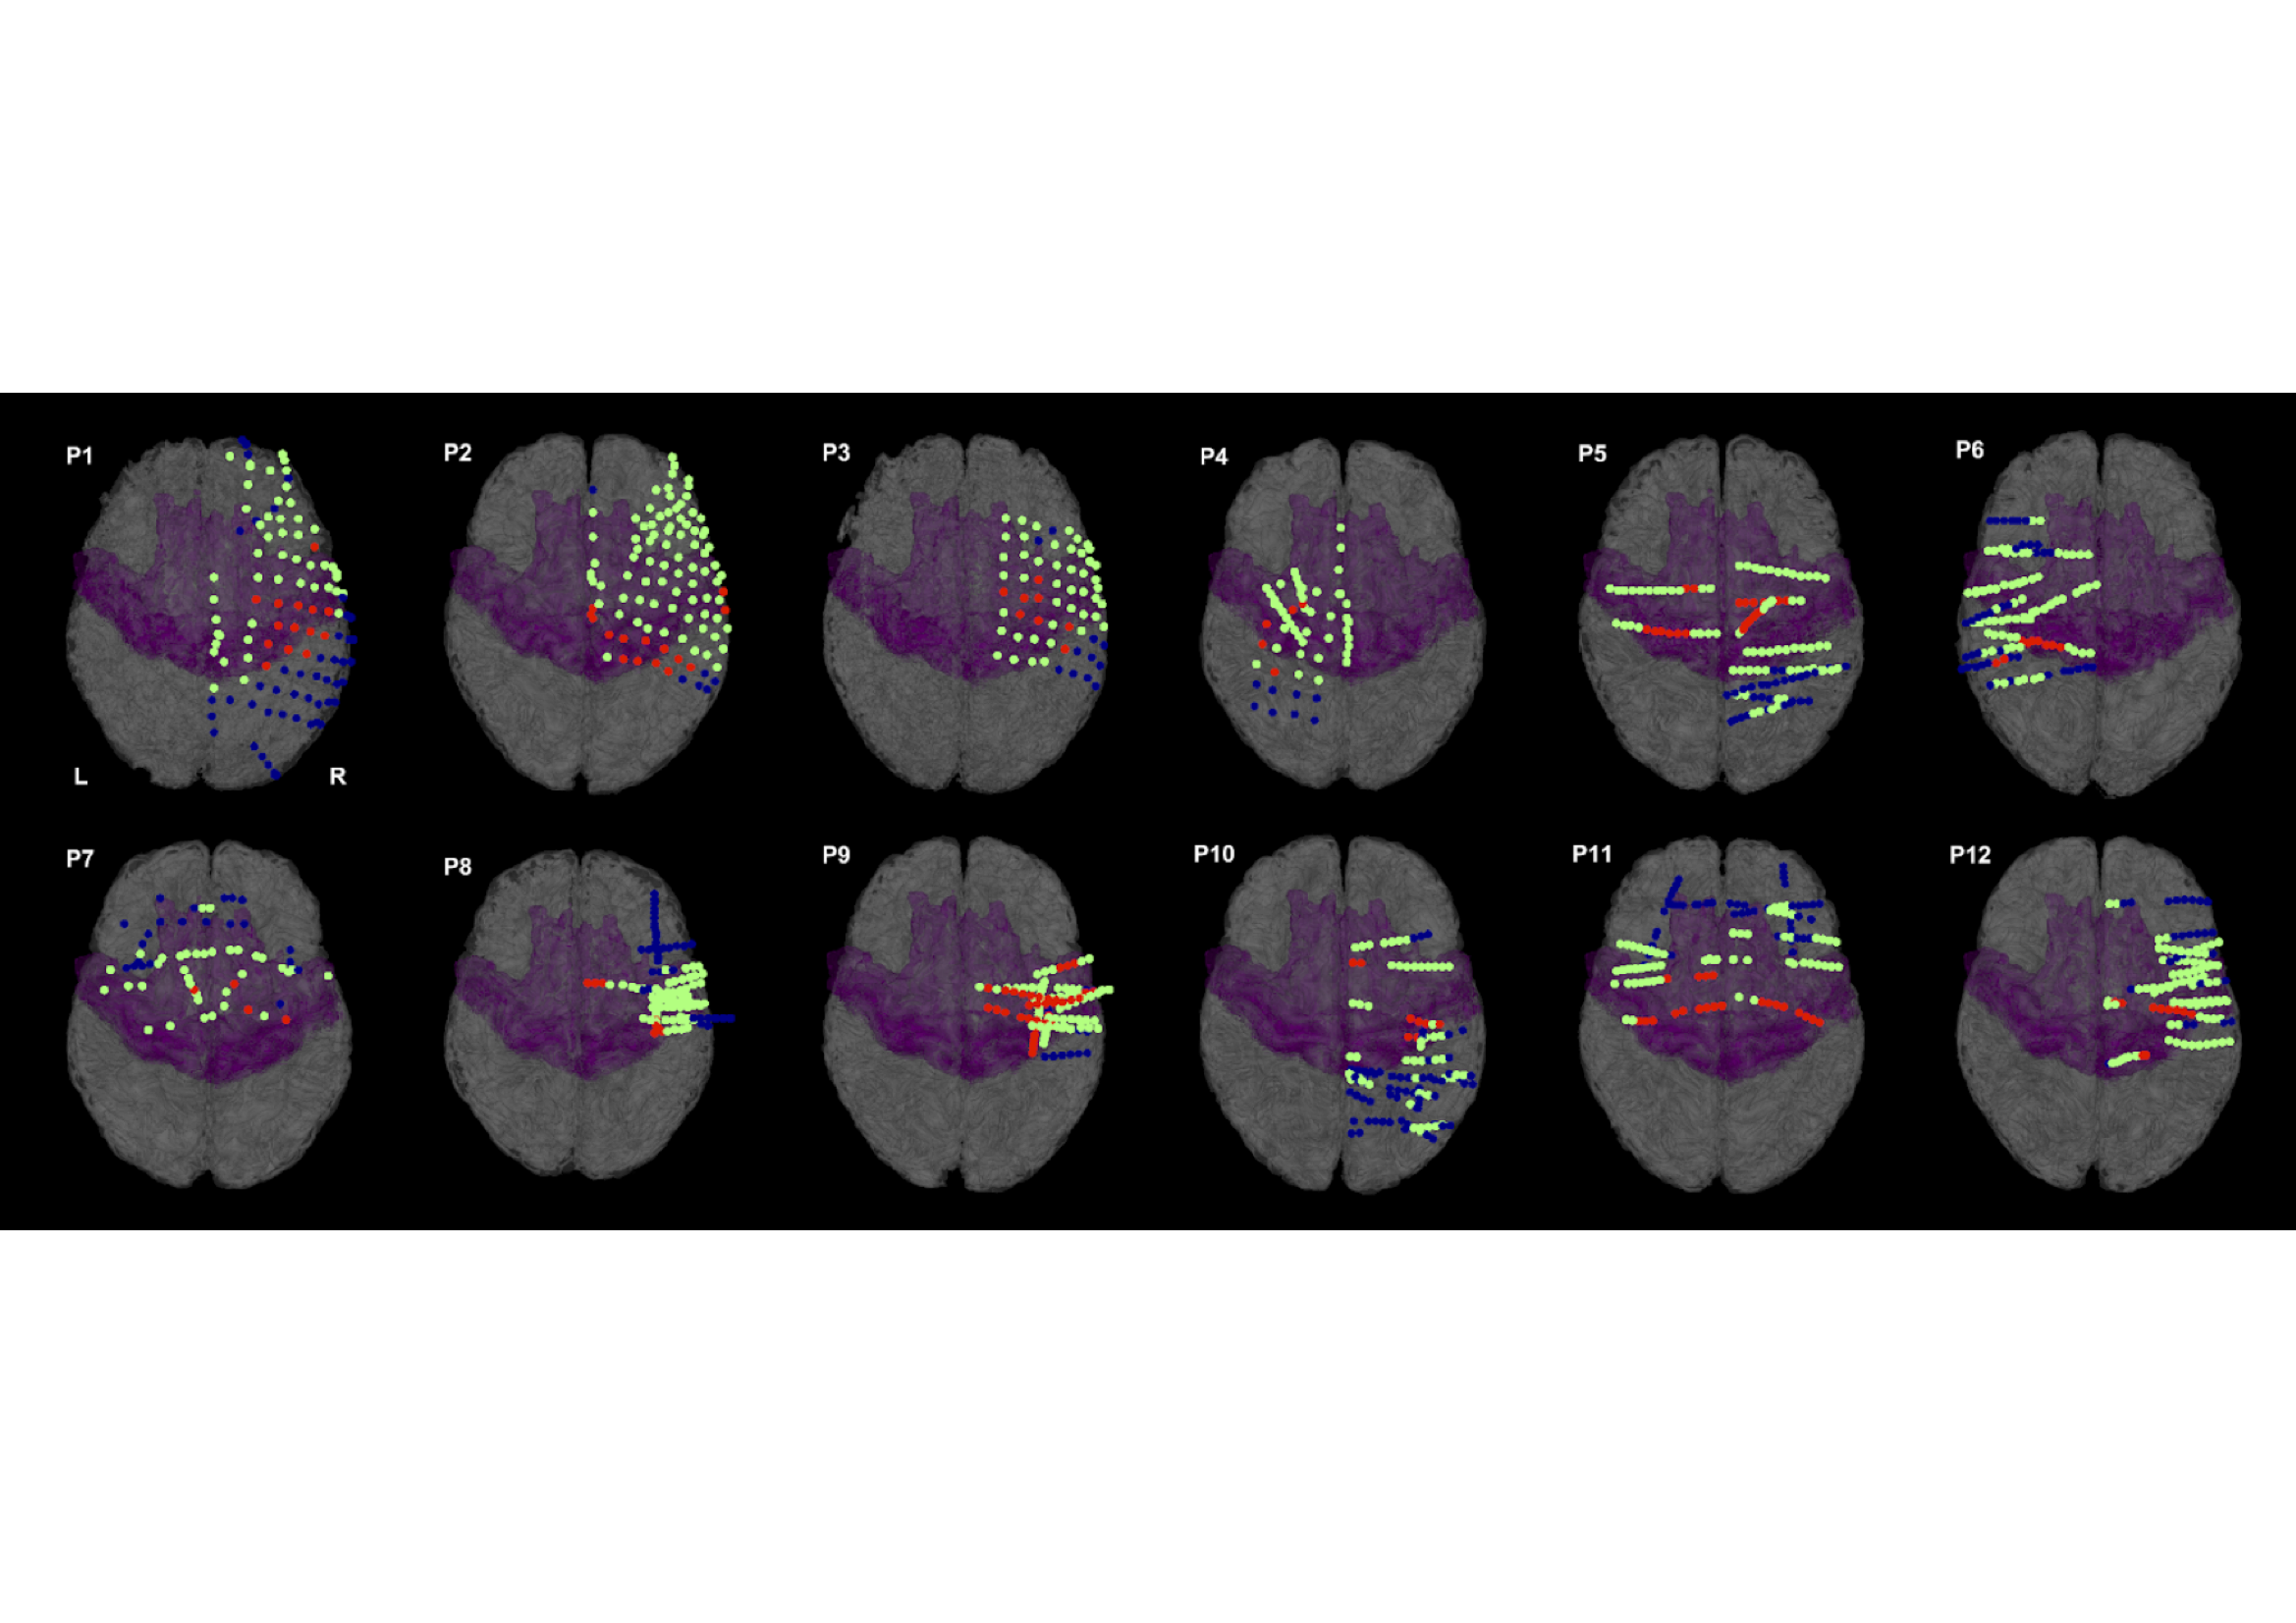
\includegraphics[width=0.8\linewidth]{img/ch3/electrodes}
\caption{Implantation schemes of the 12 patients (P1 - P12) taken from \cite{Hammer-2021}. The motor cortex is highlighted in magenta (defined as the union of areas 4 and 6 of the SPM Anatomy Toolbox). The electrodes are color-coded in the following way: Red - channels with hand-motor response after electrical stimulation mapping; dark blue - non-motor channels; green - other channels.}
\label{fig:electrodes}
\end{figure}

\begin{table}[!htbp]
\centering
\begin{tabular}{|p{1.3cm}|p{1.05cm}|p{2.15cm}|p{2.2cm}|p{1.8cm}|p{0.5cm}|p{0.65cm}|p{0.6cm}|p{0.8cm}|}
\toprule
Patient&Sex (Age)&Pathology&Implant loc&Electrode type ($N$)& $N_r$ &$N_{ch}$&$N_{m}$&$N_{nm}$ \\
\hline
\midrule
P1 & F (47) & Cryptogenic & Right frontal & ECoG (98),  sEEG (12) & 25 & 85 & 14 & 47 \\
\hline
P2 & M (48) & FCD & Right fronto-temporal & ECoG (90), sEEG (12) & 53 & 49 & 15 & 11 \\
\hline
P3 & M (50) & Cryptogenic & Right frontal & ECoG (64) & 3 & 61 & 8 & 11 \\
\hline
P4 & F (22) & FCD & Left frontal & ECoG (40),  sEEG (12) & 11 & 47 & 5 & 16 \\
\hline
P5 & F (29) & Gilosis & Left and right fronto-parietal &  sEEG (125) & 10 & 115 & 23 & 29 \\
\hline
P6 & M (29) & FCD & Left frontal &  sEEG (125) & 34 & 91 & 9 & 39 \\
\hline
P7 & F (32) & FCD & Left and right insular &  sEEG (61) & 14 & 47 & 4 & 22 \\
\hline
P8 & M (19) & FCD & Right insular &  sEEG (117) & 16 & 101 & 9 & 36 \\
\hline
P9 & F (25) & Gliosis & Right insular &  sEEG (117) & 21 & 96 & 35 & 12 \\
\hline
P10 & M (34) & FCD & Right fronto-parietal &  sEEG (125) & 23 & 102 & 8 & 63 \\
\hline
P11 & M (34) & FCD & Left and right frontal &  sEEG (126) & 11 & 115 & 21 & 48 \\
\hline
P12 & M (28) & Not operated & Right frontal &  sEEG (125) & 20 & 105 & 10 & 27 \\
\bottomrule
\end{tabular}
\caption[Patient details]{$N_r$, $N_{ch}$, $N_{m}$, $N_{nm}$  : number of rejected, non-reject, hand-motor, and non-motor channels, respectively. FCD: focal cortical dysplasia.}
\label{tab:patient-table}
\end{table}

\subsection{Separation of motor and non-motor channels}\label{subsec:separation-of-motor-and-non-motor-channels}
The separation of the channels was not a part of this thesis. 
We already obtained channels separated.
The specific separation criteria are described below as provided by Hammer et al.~\cite{Hammer-2021}. \\

One of the aims of the Hammer et al. study ~\cite{Hammer-2021} was to show what the CNNs learned from the raw brain signals.
The hypothesis was that the CNNs would focus on information from the hand-motor cortex when solving a movement-related task.
To verify this hypothesis, the recorded channels were divided into two distinct, non-overlapping groups: 1. hand-motor channels and 2. non-motor channels.
The hand-motor channels induced a clear hand motor response after the electrical stimulation at low intensities underneath or around the electrode contacts.
The non-motor channels, on the other hand, produced no sensory/motor response after the stimulation.
Furthermore, a requirement of at least 1 cm distance from the motor and pre-motor areas (i.e. Area 4a, Area 4p and Area 6 from the SPM Anatomy toolbox\cite{eickhoff-new-2005}) had to be satisfied for a channel to be included in the non-motor group.
To this end, all MRI brain scans (T1-weighted sequence) were normalized to the MNI space and the electrodes' coordinates were read out from either the post-implantation MRI or CT scans53. \\

The average number of hand-motor channels was $13 \pm 9$ ($mean \pm SD$), while there were $29 \pm 18$ ($mean \pm SD$) non-motor channels.
Some electrodes did not fall into either of the hand-motor and non-motor channel groups (e.g. channels in the motor cortex the electrical stimulation of which induced leg-motor response).
These electrodes were then left out in some analysis, because the aim was to delineate the difference between the two distinct groups of channels (the hand-motor channel group and the non-motor channel group clearly far away from the motor cortex).



\subsection{IEEG data preprocessing}\label{subsec:ieeg-data-preprocessing}
The iEEG data pre-processing was also already completed when we obtained the dataset and it was not carried out as a part of this thesis. Nevertheless, we provide the description of pre-processing from ~\cite{Hammer-2021}.
A comprehensive rejection of \textit{epileptic} channels based on the information from the respective epilepsy centers was performed, because the primary aim was to investigate the physiological brain activity.
Thus, the channels, i.e. those located in the seizure onset zone and/or containing a large number of inter-ictal epileptiform discharges, were rejected from this study ($20 \pm 13$, $mean \pm SD$ over subjects Table\ref{tab:patient-table}).
All non-rejected iEEG channels ($85 \pm 28, mean \pm SD$) were referenced to their common average, high-pass filtered at 0.15~Hz (3rd order Butterworth filter), normalized to the inter-quartile range of each channel, and resampled to 250~Hz, to yield consistent data sets from the different recording systems used at both aforementioned epilepsy centers.
The iEEG data were resampled to 250~Hz in order to emulate the same setup of the Deep4Net from~\cite{schirrmeister-deep-2017}, which was successfully applied to demonstrate high-gamma (70 - 90~Hz) effects in decoding motor behaviour from non-invasive EEG. Importantly, any over-fitting in the pre-processing was carefully avoided (i.e., all parameters of the pre-processing of the test set were estimated on the training set) and only causal, finite impulse response filters were applied.
Therefore, the decoding approach could be readily applied also in a closed-loop, online BMI. \\

The aligned iEEG and kinematic time-series were divided into 25-s long data segments.
In order to minimize a potential influence of temporal correlations in neighbouring data parts, the segments had a 2-s margins in between each other. Additionally, the last two minutes of the recordings were left as a test set. The test set was not a part of the dataset that was utilized in this thesis.


\subsection{Multiple dataset conditions}\label{subsec:modifications-to-the-dataset}
In this thesis, we refer to multiple variations of the original dataset provided by the Motol University Hospital.
Following modifications were explore: 1. filtering out certain frequencies, 2. shifting the predicted time-point with respect to the input window, 3. spectral whitening.
\begin{itemize}
\item \textbf{Filtering} We created two types of datasets using filtering.
A high-pass filtered dataset using a 15th order Butterworth filter, cut-off frequency 60~Hz, non-zero phase shift and a low-pass dataset using Butterworth filter order 15, cut-off frequency 40~Hz, non-zero phase shift. Besides full training on these datasets, parts of these datasets were combined for training and validation to see how a network trained on full data performs on high-passed data etc.
\\

\item \textbf{Shifting} Originally in Hammer et al.~\cite{Hammer-2021} the dataset was constructed so that the predictions were made from signals recorded prior to their execution (causal prediction).
In addition to this, we also created datasets where the labels (i.e. values of kinematic variables) were shifted so that predictions were made also from signals recorded after movement execution (acausal prediction).
While a network trained in this manner is unsuitable for online BCI, it allows us to inspect which time frame of the singla contains information aboout the movement.
More details about how the shift influences the predictions and why can be found in \ref{subsec:receptive-field}. \\

\item \textbf{Spectral whitening} Lastly we also created whitened datasets.
Spectral whitening normalizes amplitudes of all frequencies to one~\ref{fig:spectral-whitening}.
It was achieved using a Fourier transformation of each 25s long segment (which the dataset was divided to) into the power spectrum, obtaining information about phase and amplitude.
Then dividing the amplitudes with their absolute value and then, via inverse Fourier transformation, transforming it back to signal.
The whitened signal was normalized to its inter-quratile range (IQR).
This normalization was calculated and applied to each segment on the training set and the same parameters averaged over all 25s long segments of the training set were applied to the validation set.
\end{itemize}

\begin{figure}[!htbp]
\centering
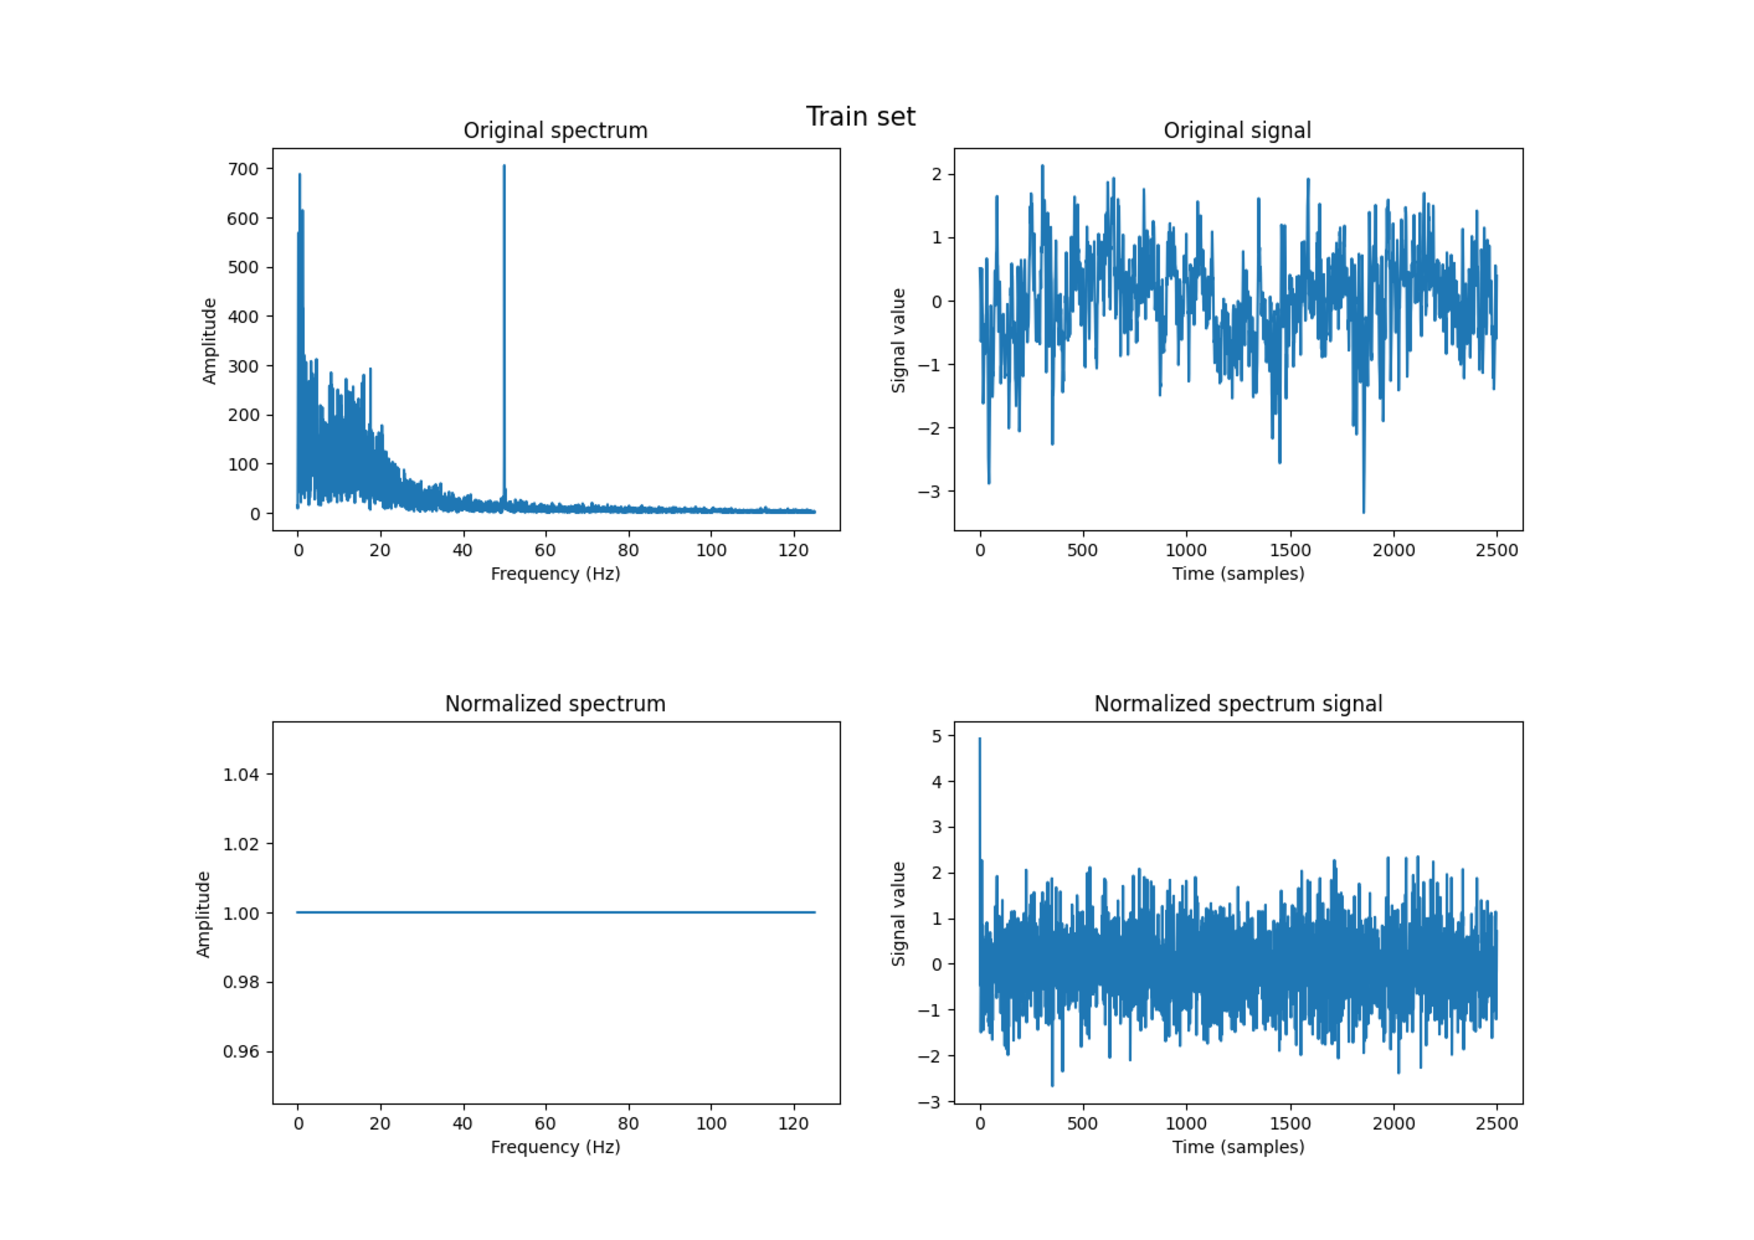
\includegraphics[width=\linewidth]{img/ch3/spectral-whitening}
\caption[Spectral whitening on the train set]{The top row shows the original power spectrum of the iEEG signal and the original iEEG signals of the first 25s long segment.
The bottom row shows how spectral whitening changed both the spectrum and the signal.}
\label{fig:spectral-whitening}
\end{figure}


\section{Deep4Net}\label{sec:deep4net}
The Deep4Net, which is freely available in the Braindecode library, was already shortly described in Section~\ref{subsec:schirrmeister-et-al}.
In this section, we describe it in more detail. 
Besides the describing the architecture as used in \cite{Hammer-2021} we focus on how cropped decoding is used \ref{subsec:cropped-decoding}, what the receptive field of the network looks like and how it affects the predictions \ref{subsec:receptive-field}, we describe the training procedure \ref{subsec:training}, the visualization of the networks gradients \ref{subsec:gradinet-visualization}, and architectural modifications we introduce in this thesis \ref{subsec:architectural-modifications}. Lastly we also state how performance is analyzed \ref{subsec:performance-analysis}.


\subsection{Architecture}\label{subsec:architecture}
The architecture which is available in the Braindecode library\footnote{https://braindecode.org} has been previously used in a number of EEG decoding tasks \cite{Hammer-2021, schirrmeister-deep-2017, hartmann-hierarchical-2018}.
It is implemented in the PyTorch framework\footnote{https://pytorch.org}.
The input of the network is a 2D array with time-steps along one axis and channels along the other axis.
The architecture consists of four convolutional-max-pooling blocks and one final convolutional filter.
It is designed so that a special first block can learn spatially global filters.
The following three standard blocks (conv\_2 - conv\_4) then allow for learning temporal hierarchies of local and global modulations~\cite{schirrmeister-deep-2017}.
The first convolutional block is split into two parts.
One performs convolution over time (conv\_temp) and the second over the channels with weights for all possible electrode pairs using filters of the preceding temporal convolution (conv\_spat).
Because there is no activation function between these two layers, they could be merged, but the authors emphasize the regularization function of this separation because it forces a separation of the linear transformation into a temporal convolution and a spatial filter. \\

The convolutional blocks start with a convolutional layer, then a batch normalization layer follows, after which a non-linearity is added, in the case of the Deep4Net it is the exponential linear unit (ELU) function\cite{clevert-elu-2016}.
Finally a max-pool layer closes the convolutional block.
An output layer, which is a softmax, comes last.
To use this network for regression task that the present thesis focuses on, only a single modification needs to be done: removing the last softmax layer and replacing it with a convolution (conv\_classifier).
The architecture already transformed for regression is depicted in Figure~\ref{fig:architecture}. \\

The Deep4Net is able to process varying input shapes.
In each convolutional layer it simply slides its filters over the input and gives a respective number of outputs.
Therefore, before training, the number of outputs needs to be calculated based on the size of the input window that was chosen.
The corresponding values of the predicted kinematic variables are cropped accordingly.
In this thesis, we used 1200 samples as input which corresponds to 4.8 seconds in time.
For the Deep4Net a window of 1200 samples gives 679 predictions.
Therefore, one prediction is made from $11200 - 679 + 1 = 522 $ samples measured before execution which translates to 2.088 seconds.
This is consistent with Hammer et al. \cite{Hammer-2021} where they used 2 second long segments.
Importantly to note, in Hammer et al. \cite{Hammer-2021} and also for the most part in this thesis, the input window predicting a time-point was shifted so that all the information used to decode this time-point happened prior to movement execution.
This makes the network suitable for online BCI\@. \\

Lastly we point out, that the network does not use any padding. 
This makes its receptive field non-uniform but is necessary to perform cropped decoding described in Section \ref{subsec:cropped-decoding}.

\begin{figure}[!htbp]
\centering
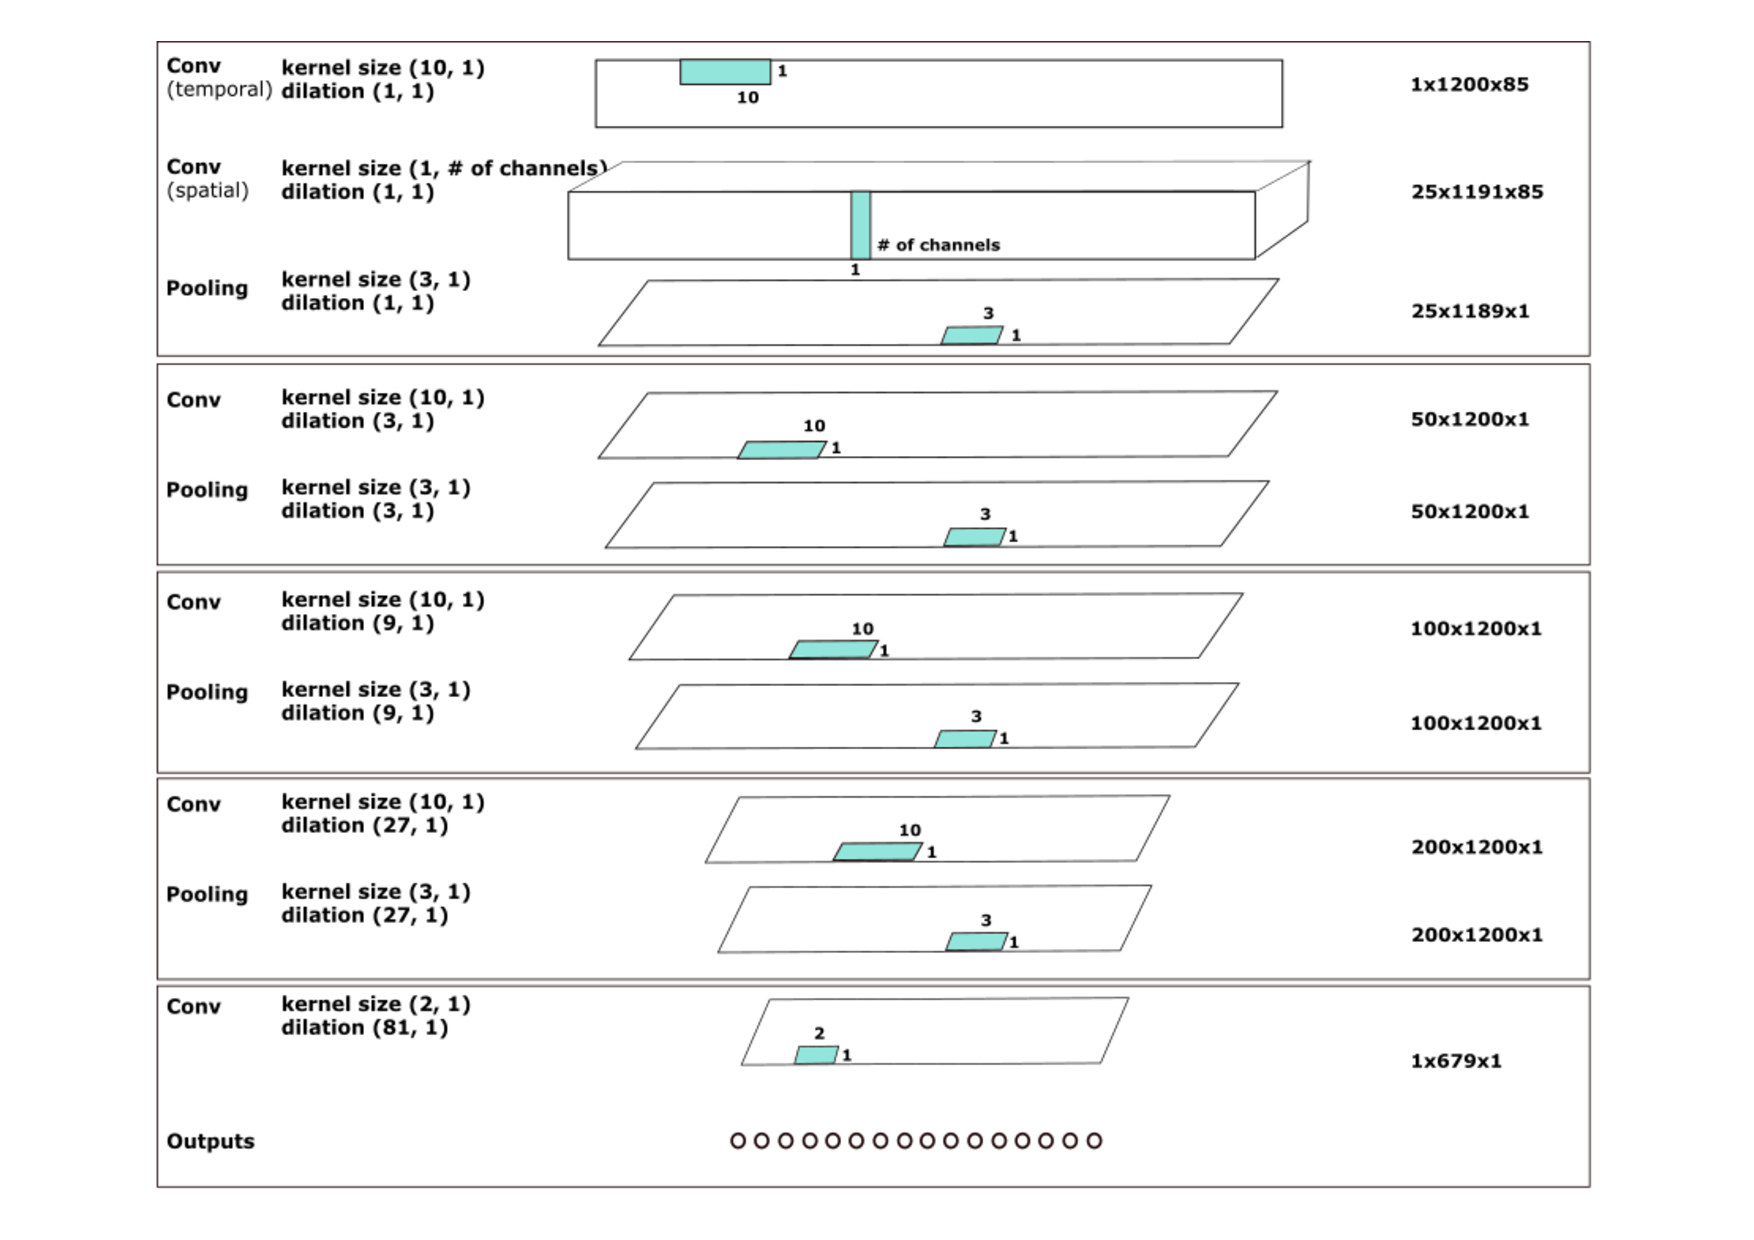
\includegraphics[width=\linewidth]{img/ch3/architektura}
\caption[Deep4Net]{The architecture of the Deep4Net modified to be suitable for regression as used in \cite{Hammer-2021}}
\label{fig:architecture}
\end{figure}

\subsection{Cropped decoding}\label{subsec:cropped-decoding}
The possibility to use cropped decoding is implemented the Braindecode library together with the original Deep4Net.
Instead of giving one trial and obtaining one prediction, the trial window is separated into multiple smaller overlapping sub-windows each of which produces a prediction.
In case of classification, these multiple outputs for one input window are then averaged to give the final prediction from which loss is calculated Figure~\ref{fig:trial-wise-decoding}.


\begin{figure}[!htpb]
\centering
\begin{subfigure}[b]{0.4\textwidth}
   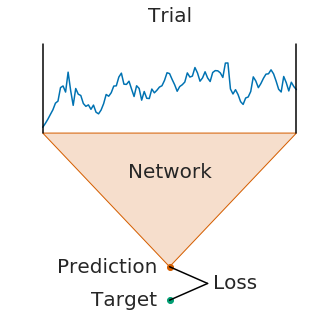
\includegraphics[width=0.9\linewidth]{img/ch3/trialwise-explanation.png}
   \caption{Trial-wise decoding}
   \label{fig:trial-wise-decoding-trial-wise}
\end{subfigure}

\begin{subfigure}[b]{0.55\textwidth}
   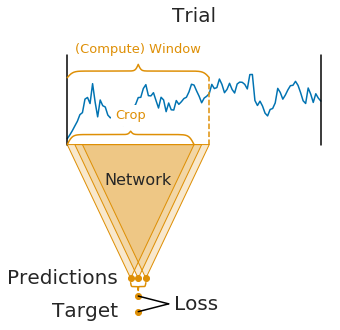
\includegraphics[width=0.9\linewidth]{img/ch3/trialwise-explanation2.png} 
   \caption{Cropped decoding}
   \label{fig:trial-wise-decoding-cropped}
\end{subfigure}
\caption[Trial-wise vs. cropped decoding]{This Figure obtained from the Braindecode library documentation\footnote{https://robintibor.github.io/braindecode/notebooks/Cropped\_Decoding.html} illustrates the difference between cropped decoding and trial-wise decoding for classification.}
\label{fig:trial-wise-decoding} 
\end{figure}

To avoid a longer training time, Schirrmeister et al.\cite{schirrmeister-deep-2017} also introduced a feature with dilated convolution.
It was previously also implemented for speeding up CNNs that make predictions for each pixel of an image \cite{}. 
This speed-up requires changes in the architecture.
In order to implement a network which can process multiple crops at the same time and give an equivalent result as the network processing one crop at a time, the strides of the layers can be removed (set to 1) and instead replaced by an increasing dilation.
A visual explanation of this is in Figure \ref{fig:cropped-decoding-scheme}.

\begin{figure}[!htbp]
\centering
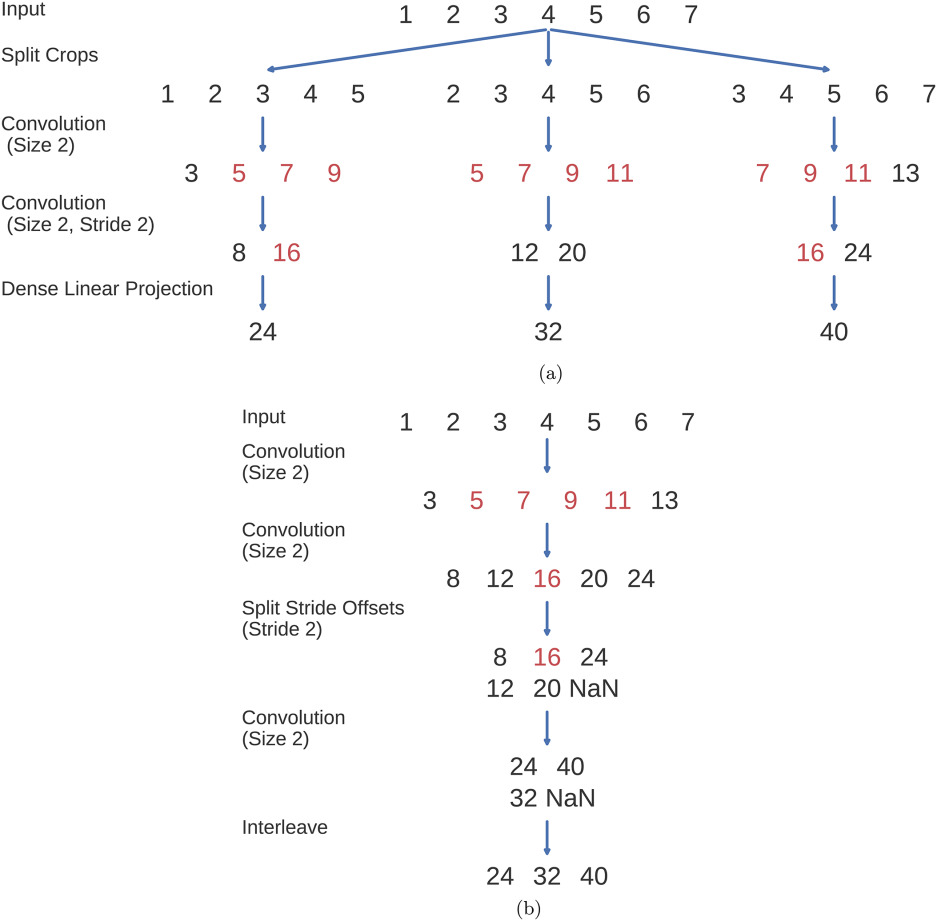
\includegraphics[width=\linewidth]{img/ch3/cropped-decoding-scheme}
\caption[Processing crops]{A toy example from \cite{schirrmeister-deep-2017} presenting the difference between \textbf{a)} the naive approach to process crops using a network with strides; and \textbf{b)} processing crops at the same time using the dilated network}
\label{fig:cropped-decoding-scheme}
\end{figure}

The algorithm used to make the transition between strides and dilations is described in Algorithm\ref{alg:stride-to-dilation}.

Algorithm~\ref{alg:stride-to-dilation} describes how a network with stride is converted into a network with dilations.\\
\begin{algorithm}
\begin{lstlisting}[language=Python,label={lst:lstlisting}]
def to_dense_prediction(network):
	current_stride = 1
	for module in network.modules:
		if hasattr(module, 'dilation'):
			module.dilation = current_stride
		if hasattr(module, 'stride'):
			current_stride *= module.stride
			module.stride = 1
\end{lstlisting}
\caption{The simplified algorithm used to transform a network with strides to a network with dilations in the Braindecode library.
This version assumes a 1D stride and dilation which is sufficient for our case as all the strides in the networks are 1D.
}
\label{alg:stride-to-dilation}
\end{algorithm}

The algorithm allows us to transform every network with stride and without right padding, into an equivalent network with dilations (dilated network).
Right padding would disrupt the equivalency of computation.
Nevertheless, this transformation relationship is not symmetric.
For some dilated networks no networks with strides without right padding performing an equivalent trial-wise computation exist.
An example of such a network is a CNN where in two consecutive layers with a dilation parameter, the first layer has bigger dilation than the second one.
This cannot happen if we follow the algorithm above~\ref{alg:stride-to-dilation} thus, such a CNN was not derived from a CNN with strides. \\

In Schirrmeister et al.~\cite{schirrmeister-deep-2017} where the Deep4Net originated the architectures were constructed in the space of the CNNs with stride which were then converted into dilated networks.
This leaves a whole set of architectures unexplored.
Namely, those dilated networks which cannot be constructed from a CNN with stride.
These dilated networks cannot be used for trial-wise decoding.
Nevertheless, this is no drawback for our task at hand because we .


\subsection{Receptive field}\label{subsec:receptive-field}
The fact that the Deep4Net cannot have right padding in order to process multiple windows at the same time affects its receptive field.
By receptive field we mean the space of the input of the network which affects one specific output.
In \cref{fig:receptive-field} we visualize the receptive field used for one prediction.
The figure illustrates how many times each input sample (including the values derived from it) is used in a forward pass through the CNN to obtain the specific prediction.
Note, that the receptive field in no way illustrates the weights of the network.

\begin{figure}[!htbp]
\centering
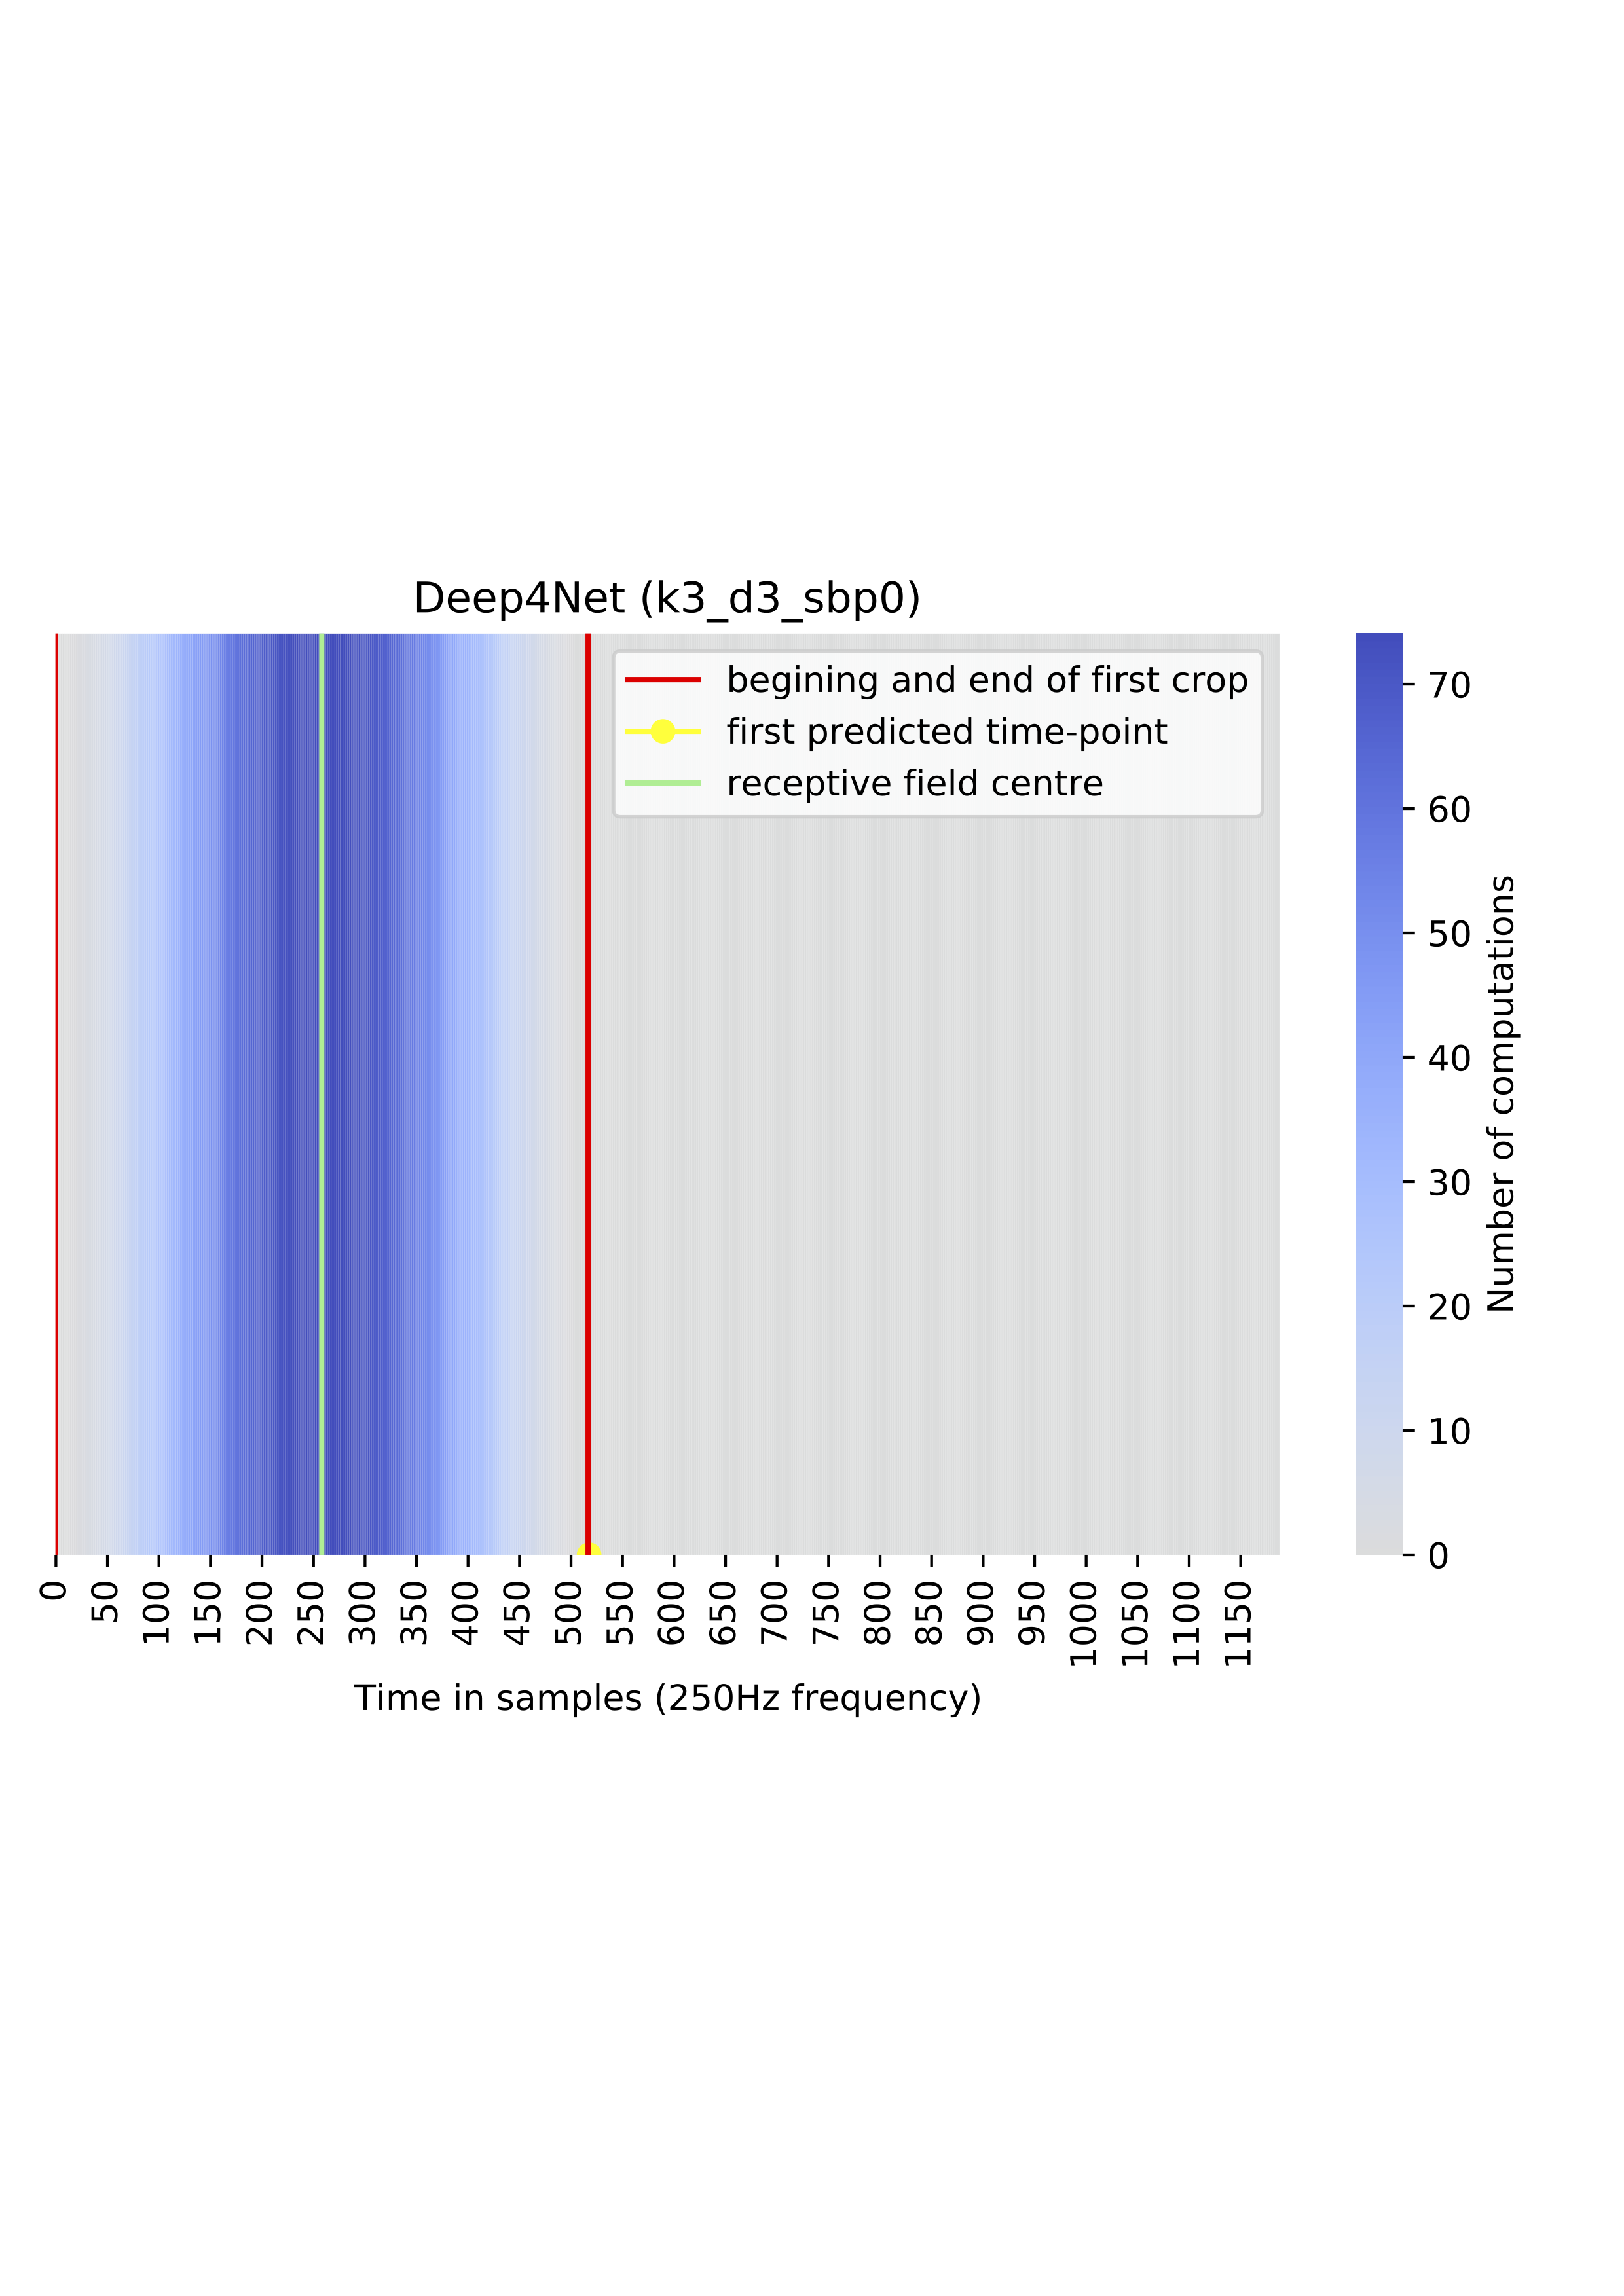
\includegraphics[width=0.8\linewidth]{img/ch3/deep4net-receptive-field}
\caption[Receptive field]{The receptive field of the original Deep4Net, which is the base model derived from \cite{Hammer-2021}, in this thesis denoted as {variable}\_k3\_d3\_sbp0.
The vertical red lines delimit the first receptive field (crop) of the CNN which is used for calculating the first prediction.
The whole 
The green line represents the centre of the receptive field and the yellow dot on the x axis the first time-point that is being predicted. The gradient bar on the right shows the number of times each input sample was used in the calculations of the output.}
\label{fig:receptive-field}
\end{figure}

Figure~\ref{fig:receptive-field} illustrates that the predicted time-point is fairly far from the centre of the receptive field.
This is because we make the prediction only based on the data recorder prior to the predicted movement.
The receptive field at the time-point where the prediction is made.
But the CNN mostly focuses on signals around the centre of the receptive field and therefore, is biased towards data are far from those that directly precede the movement. \\

For classification this is not as critical, because the same label is predicted from multiple crops, and the actual classified movement does not happen at the end of the last crop but at some point during the whole input window from which the crops are derived \cite{schirrmeister-deep-2017}.
This gives the network a chance to focus on information directly preceding the actual movement. \\

We focus on the changed role of the receptive field between classification and regression because as previously stated in \cite{schirrmeister-deep-2017, hartmann-hierarchical-2018}, this same CNN architecture was shown to utilize information from the high-gamma frequency bands. 
Since we are investigating the frequency bands and their effective utilization, we inspect this difference as a possible reason the network when employed to do regression does not use high-gamma.
The hypothesis here is, that the high-gamma signal is most informative directly before the movement execution.
Therefore, the distance of the network's receptive field centre to the predicted time-point hinders its usage.
We test this hypothesis in the \cref{sec:shifting-the-predicted-time-point}.

\subsection{Training}\label{subsec:training}
Except for the learning rate, we left all hyper-parameters equal to those from Hammer et al. \cite{Hammer-2021}, because it was our goal to reproduce their results and build up on their research.
The network was trained for 100 epochs with batch size 32, using Adam~\cite{kingma-adam-2017} as the optimizer and learning rate 0.001.
The reported learning rate in Hammer et al. was 0.01.
However, we used a lower learning rate because otherwise, the results were significantly worse than reported in Hammer et al. \\

For each patient separately, the 25s-long segments were divided into 5 equal or almost equal subsets and a 5-fold cross-validation was performed to estimate decoding accuracy.
The number of these segments varied among patients.
Therefore, the dataset sizes varied across models for different patients but the ratio was kept the same 80-20 training-validation.
In Hammer et.\ al, they performed leave-one-out cross-validation on the 25s-long segments.
Nevertheless, with the amount of different architecture and modified datasets we explored, this would be extremely time consuming.
Performing 5-fold cross-validation gives us a good estimation of the networks' performances while also saving computational power.

\subsection{Gradient visualization}\label{subsec:gradinet-visualization}
The gradient visualization algorithm is the following.
First, the input signal is converted into the power spectrum using Fourier transformation.
After this transformation, hooks are created for the amplitude and phase values.
Then it is converted back into the original signal, this time using the torch functions so PyTorch can start building its computational graph reaching back to the amplitudes and phases.
This tracked signal is then given to the network, whose weights are frozen, as input.
After obtaining the outputs, the outputs are averaged and the \texttt{torch.autograd.backward()} function is used to derive the gradients with respect to the frequency amplitudes and phases \cite{gradient-visualization}. \\

Throughout the thesis, the input window used in the above described algorithm was set to twice the size of the receptive field of the network to be consistent with \cite{Hammer-2021}.
A special case is the gradient visualization when the input window is shortened so that the network has only one output was also explored as a part of this thesis.
See section \ref{sec:gradient-peak}.
In this special case, the outputs did not have to be averaged before using the \texttt{torch.autograd.backward()} function to derive the gradients. \\

To obtain representative gradients, the above described procedure is always repeated over multiple batches for each patient and the resulting gradients are averaged.
Gradients are useful in showing, to modulations in which frequencies the network reacts more strongly. 
The higher gradient value for a certain frequency, the more the change is this frequency influences the prediction. \\
 
Because there are no significant differences between the gradients of the networks on the training set and the validation set we chose to always display the gradient values for the training set.
Also note that in this thesis we only address the gradients for the frequency amplitudes.
While inspecting the phase gradients would also be interesting, it is out of the scope of this thesis.


\subsection{Architectural modifications}\label{subsec:architectural-modifications}
During our research, we made a set of modifications to the architecture of the Deep4Net creating multiple new CNNs.
With our changes we focused on the kernel sizes and dilation parameters of the four max-pool layers present in the network.
Table~\ref{tab:architectures-description} explains the terminology used with respect to the max-pool parameters used throughout the thesis.
The original Deep4Net corresponds to the {variable}\_k3\_d3\_sbp0 in Table\ref{tab:architectures-description}.
The suffix \textit{sbp} refers to a parameter of the Deep4Net namely the \texttt{stride\_before\_pool} parameter.
This parameter influences the dilations in the max-pool layers of the network.
For a visual explanation of dilation see \ref{fig:dilation}.
In Hammer et al~\cite{Hammer-2021} and Schirrmeister et al. \cite{schirrmeister-deep-2017}this parameter was set to \texttt{False (sbp0)}, nevertheless, some analyses performed by their group which we are referring to in Section \cref{sec:gradient-peak}, the studied network had \texttt{stride\_before\_pool} set to \texttt{True (sbp1)}. \\

Therefore, we focus on the Deep4Net with \texttt{sbp1} in Section \ref{sec:gradient-peak} but the default Deep4Net architecture is the one with \texttt{sbp0} as in Hammer et al. For the other CNNs we created, this parameter becomes meaningless because we manually set the sizes of the dilations for all the max-pool layers with no consideration of this parameter. \\



When we change the parameters of the max-pool layers as we describe above, the number of outputs the network has changes.
It also causes changes in the receptive field of the network.
To see how, consider just one max-pool layer with dilation 3 (L3) and one max-pool layer with dilation 1 (L1). 
If we use a window of the same length as input for L3 and L1 and compare the dimensions of the outputs from these layers, the dimension of the output of L3 will be smaller than of the L1.
\todo{illustration of this}.
Consequently, if we alter the dilation (and also kernel) parameters of the max-pool layers in the Deep4Net, we get a different number of outputs from the altered network.  \\

When one network has dilations 1, 3, 9 and 27 in the max-pool layers (the k*\_d3) and the other one 1, 1, 1 and 1 (k*\_d1), the difference in the dimension of the output is significant.
The latter network makes more predictions from the same input length because the dimension of the output is larger.
It also has a smaller receptive field for one prediction as is visulalized in~\cref{fig:receptive-field-comparison}.
Information about the size of the receptive field can also be found in Table~\ref{tab:architectures-description}.

\begin{figure}[!htpb]
\centering
\begin{subfigure}[b]{0.44\textwidth}
   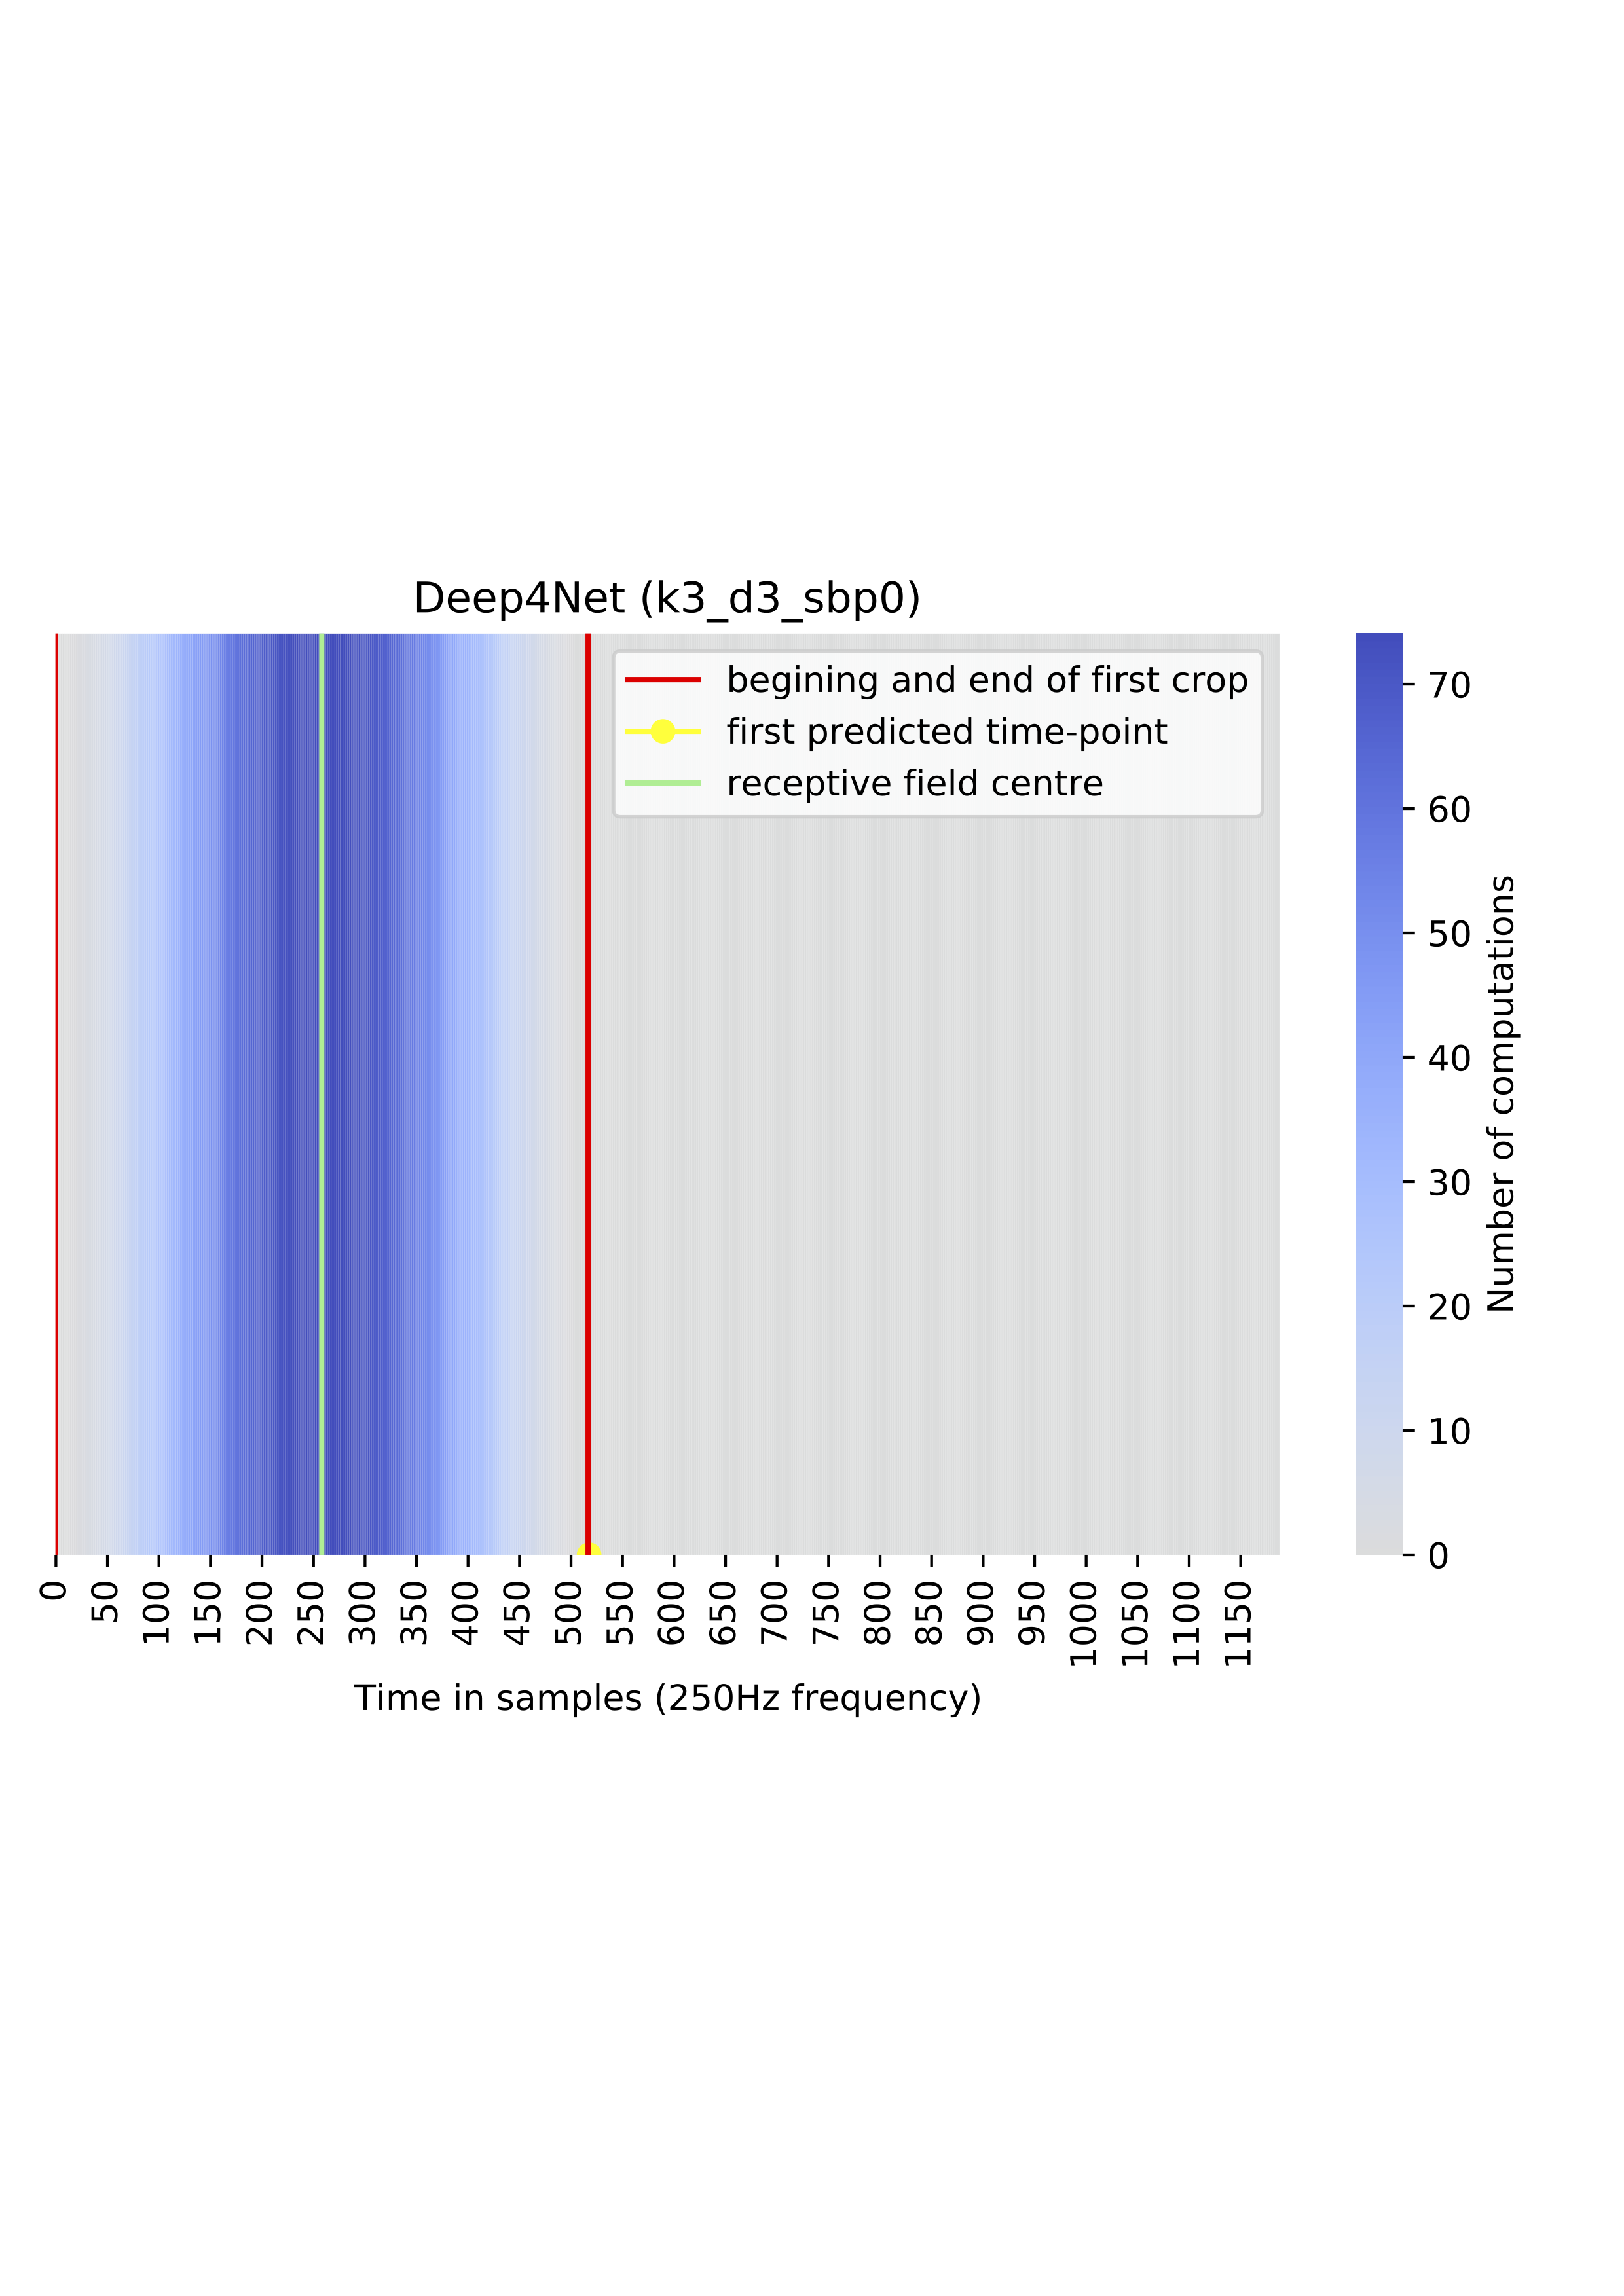
\includegraphics[width=\linewidth]{img/ch3/deep4net-receptive-field}
   \caption{Receptive field of the Deep4Net (k3\_d3\_sp0).}
\end{subfigure}
\begin{subfigure}[b]{0.44\textwidth}
   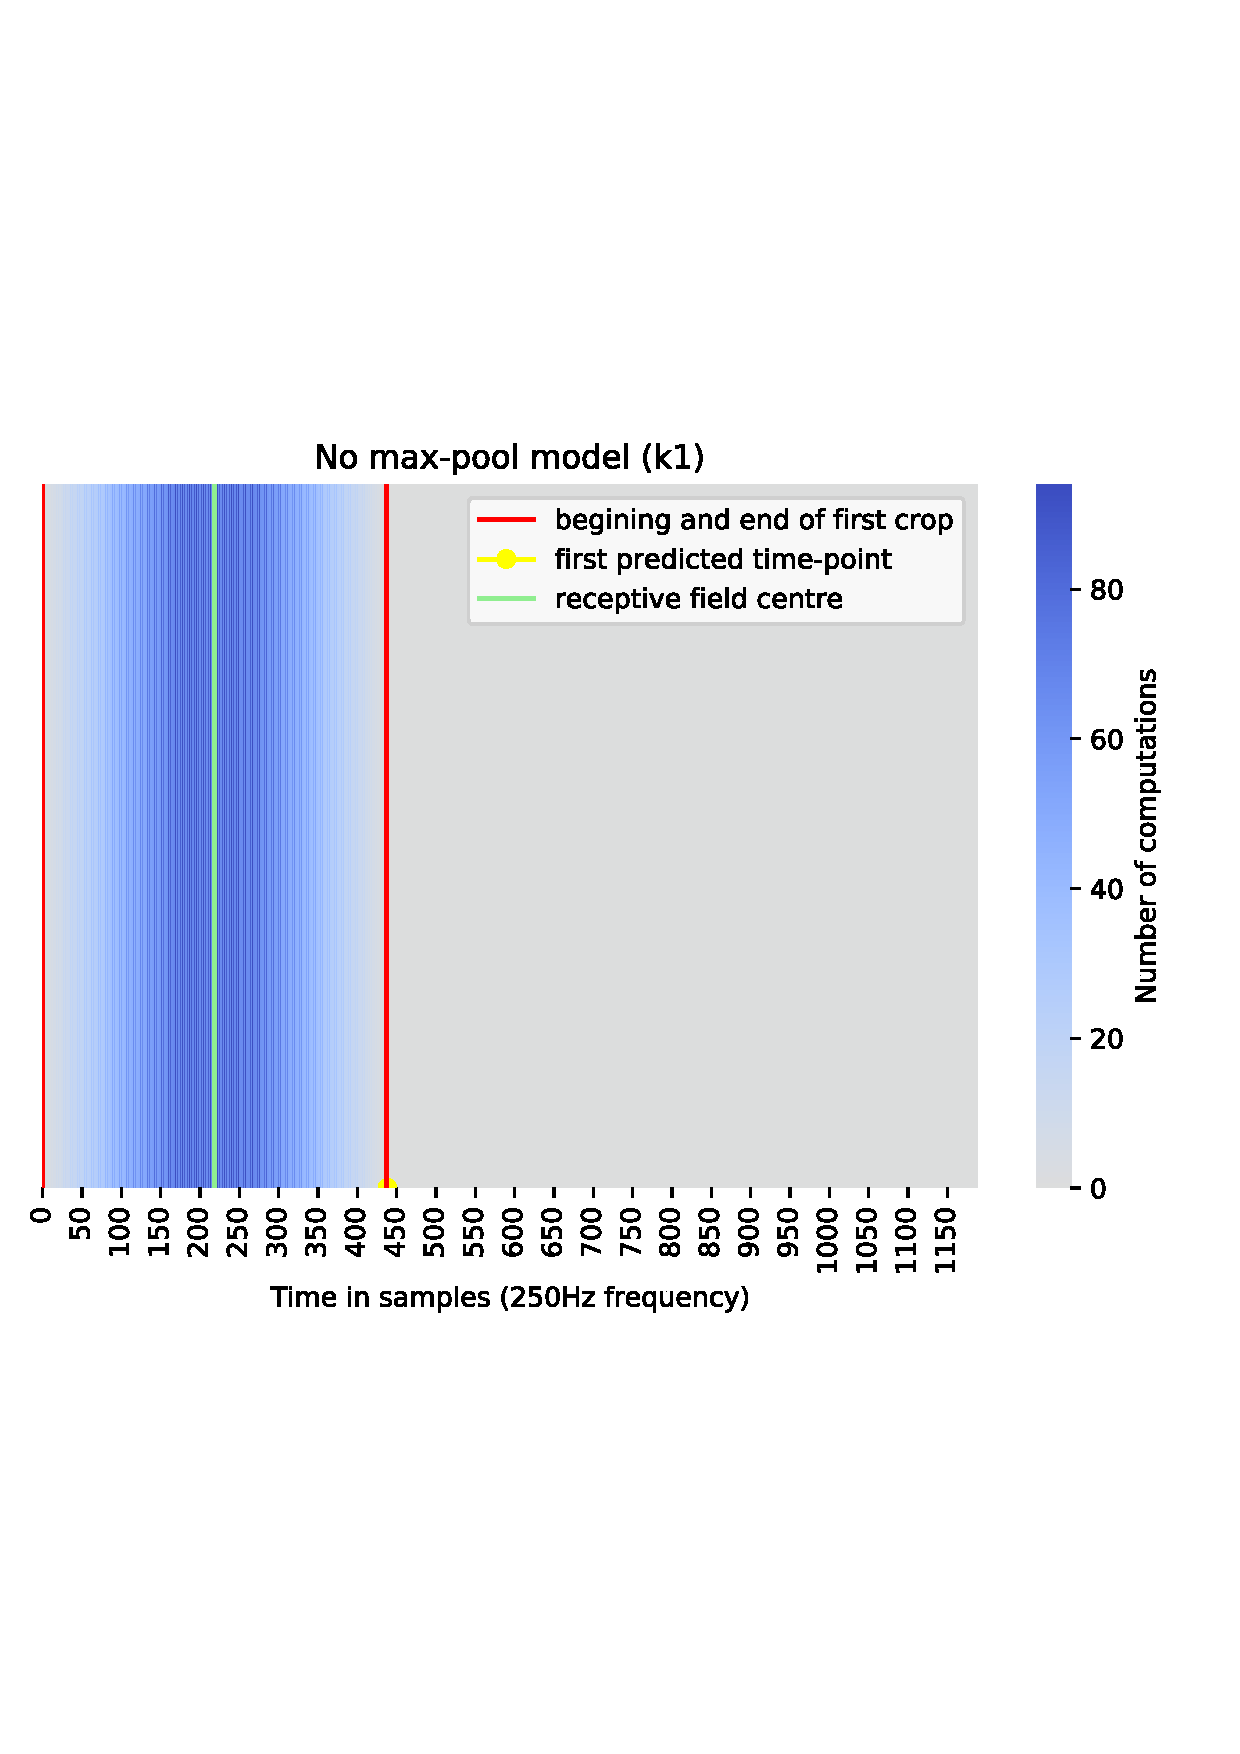
\includegraphics[width=\linewidth]{img/ch3/k1-receptive-field}
   \caption{Receptive field of the CNN without max-pool (k1).}
\end{subfigure}
\caption[Receptive field comparison]{Both graphs \textbf{(a)} and \textbf{(b)} show the receptive field used for making one prediction (delimited by red lines) with respect to one complete 1200 ms long input window which is given to the networks. The receptive field in \textbf{(b)} is smaller, reaching to less than 450, where as the receptive field of \textbf{(a)} reaches beyond 500.} 
\label{fig:receptive-field-comparison}
\end{figure}

\begin{table}[!htpb]
\centering
\begin{tabular}{|p{3.7cm}|p{1.7cm}|p{2cm}|p{1.2cm}|p{2.5cm}|}
\toprule
Model name & Max-pool kernel size & Max-pool dilations & Stride before pool & Size of the receptive field \\
\midrule
variable\_k1 & 1, 1, 1, 1 & -- & -- & 442 samples \\
\hline
variable\_k2\_d3 & 2, 2, 2, 2 & 3, 9, 27, 81 & -- & 562 samples \\
\hline
variable\_k3\_d3\_sbp1 & 3, 3, 3, 3 & 3, 9, 27, 81 & True & 682 samples \\
\hline
variable\_k3\_d3\_spb0 & 3, 3, 3, 3  & 1, 3, 9, 27 & False & 522 samples \\
\hline
variable\_k2\_d1 & 2, 2, 2, 2 & 1, 1, 1, 1 & -- & 446 samples \\
\hline
variable\_k3\_d1 & 3, 3, 3, 3  & 1, 1, 1, 1 & -- & 450 samples \\
\hline
variable\_k2\_d2 & 2, 2, 2, 2 & 2, 4, 8, 16 & -- & 472 samples \\
\hline
variable\_k3\_d2 & 3, 3, 3, 3 & 2, 4, 8, 16 & -- & 502 samples \\
\hline
\bottomrule
\end{tabular}
\caption[Architectural modifications]{This table gives an overview of the various CNN architectures we investigated in the scope of this thesis. Modifications were always made to the last four convolutional layers. The two convolutions in the first convolutional block (i.e. the spatial and spectral convolutions) stayed the same for all CNNs. Only information about the first dimension of the kernel sizes and dilations is presented. The second dimension is always 1. I.e. Max-pool kernel sizes 2, 2, 2, 2 actually represent kernel sizes of conv\_2, conv\_3, conv\_4 and conv\_classifier being (2, 1), (2, 1), (2, 1), (2, 1). }
\label{tab:architectures-description}
\end{table}

\subsection{Performance analysis}\label{subsec:performance-analysis}
When comparing two models, we are not comparing them based on the mean-square error (MSE) which is the loss function of the training, but on the correlation coefficient (CC) between the model's predictions and the predicted kinematic variable.
Specifically the Pearson's correlation coefficient \cite{pearson-vii-1895}.
Often throughout the thesis we show boxplots of CCs of different architectures.
Each boxplot is obtained from performing a 5-fold cross-validation for each of the 12 participants.
The results from the 5 folds are averaged and the box-plot is created from the 12 averages.
While it is possible to create the box-plots from all the folds and not averaging them for each patient, we are interested in the distribution of correlation among patients rather than among individual runs.